% ====================================================================
%+
% SECTION:
%    section-name.tex  % eg lenstimedelays.tex
%
% CHAPTER:
%    chapter.tex  % eg cosmology.tex
%
% ELEVATOR PITCH:
%    Explain in a few sentences what the relevant discovery or
%    measurement is going to be discussed, and what will be important
%    about it. This is for the browsing reader to get a quick feel
%    for what this section is about.
%
% COMMENTS:
%
%
% BUGS:
%
%
% AUTHORS:
%    Phil Marshall (@drphilmarshall)  - put your name and GitHub username here!
%-
% ====================================================================

\section{Disc Intrinsic AGN Variability}
\def\secname{\chpname:variability}\label{sec:\secname}

\credit{ohadshemmer},
\credit{vpk}
{\it and others to follow}

% This individual section will need to describe the particular
% discoveries and measurements that are being targeted in this section's
% science case. It will be helpful to think of a ``science case" as a
% ``science project" that the authors {\it actually plan to do}. Then,
% the sections can follow the tried and tested format of an observing
% proposal: a brief description of the investigation, with references,
% followed by a technical feasibility piece. This latter part will need
% to be quantified using the MAF framework, via a set of metrics that
% need to be computed for any given observing strategy to quantify its
% impact on the described science case. Ideally, these metrics would be
% combined in a well-motivated figure of merit. The section can conclude
% with a discussion of any risks that have been identified, and how
% these could be mitigated.

% A short preamble goes here. What's the context for this science
% project? Where does it fit in the big picture?

A variety of AGN variability studies will be
enabled by LSST. These are intended to probe the physical properties
of the unresolved inner regions of the central engine. Relations will
be sought between variability amplitude and timescale vs. $L$, $z$,
$\lambda_{\rm eff}$, color, multiwavelength and spectroscopic
properties, if available. The LSST sampling is expected to provide
high-quality power spectral density (PSD) functions for a large number
of AGNs; these can be used to constrain the SMBH mass and accretion
rate/mode. Furthermore, LSST AGNs exhibiting excess variability over
that expected from their luminosities will be further scrutinized as
candidates for lensed systems having unresolved images with the excess
(extrinsic) variability being attributed mainly to microlensing.

Potentially periodic AGN variability, leading to tentative discoveries
of binary SMBHs (e.g., \citet{GrahamEtal2015}), may also be
measurable.  Over the ten-year survey, LSST will be sensitive to
periods of a few days up to $\sim3$~yr.

Photometric reverberation mapping (PRM), measuring the time-delayed
response of either the flux of the broad emission line region (BELR)
lines to the flux of the AGN continuum or between the continuum flux
in one (longer wavelength) band to the continuum flux in another (band
with shorter wavelength), will be one of the cornerstones of AGN
research in the LSST era (e.g., \citet{Chelouche2013};
\citet{CheloucheandZucker2013}; \citet{CheloucheEtal2014};
\citet{EdelsonEtal2015}; \citet{FausnaughEtal2015}). For example, LSST
is expected to deliver BELR line-continuum time delays in
$\sim10^5-10^6$ sources, which is unprecedented when compared to
$\sim50-100$ such measurements conducted via the traditional, yet much
more expensive (per source) spectroscopic method. Sources in the
deep-drilling fields (DDFs) will benefit from the highest quality PRM
time-delay measurements given the factor of $\sim10$ denser sampling.


Regarding QPOs:
1) The QPO periods expected from the inner accretion disk (which provide
 a stable clock which is located closer to the horizon as the BH spin
  increases) can be estimated from that of the fundamental g-mode, which agree
   with the observed QPO frequencies in stellar mass BH binaries. Utilizing the
    theoretical upper bounds for BH spin and $L/L_{\rm Edd}$, and the lower bound
     to the $k$- and bolometric correction $B_i(Z)$ , one obtains
 $\log P(hours) > 0.4(1-m_i) + \log[(1+Z)D(Z)^2]$
for i-band magnitude $m_i$ and luminosity distance $D(Z)$. $B_i(Z)$ is a decreasing 
function of BH mass, but an increasing function of BH spin.
2) The Lyman-alpha forest limits us to redshifts $Z < 2.7$ in the g-band. The QPO 
will be weaker within longer wavelength bands.
3) The $\sim 80$ visits in the g-band proposed for the main survey appears 
insufficient to produce a useful PSD.
4) The expected QPO periods are longer than a few hour visit in a DDF. For instance,
 for $m_g  <  23$ and the optimal $Z =  2.7$, the QPO period P > 4 hours.

QPO search will be most relevant for the DDFs, if the sampling is at least ~nightly, i.e., ~3000 visits
during the entire survey. In addition, there's a need for an "ultradeep" field, e.g., the MCs, that will
be monitored, during commissioning phase, with frequencies in the range ~$1$-$10^4$ min. (i.e., from
minutes to weeks/months).

% --------------------------------------------------------------------

\subsection{Target measurements and discoveries}
\label{sec:\secname:targets}

We will measure the power spectral density (PSD) of AGN light 
curves across $L$, $z$, and $\lambda_{\rm eff}$. Specifically, we will
 measure the short timescale ($\leq 5$~d) spectral index of the PSD and
 the locations of `features' such as QPOs
 and breaks in the PSD.

\begin{figure}
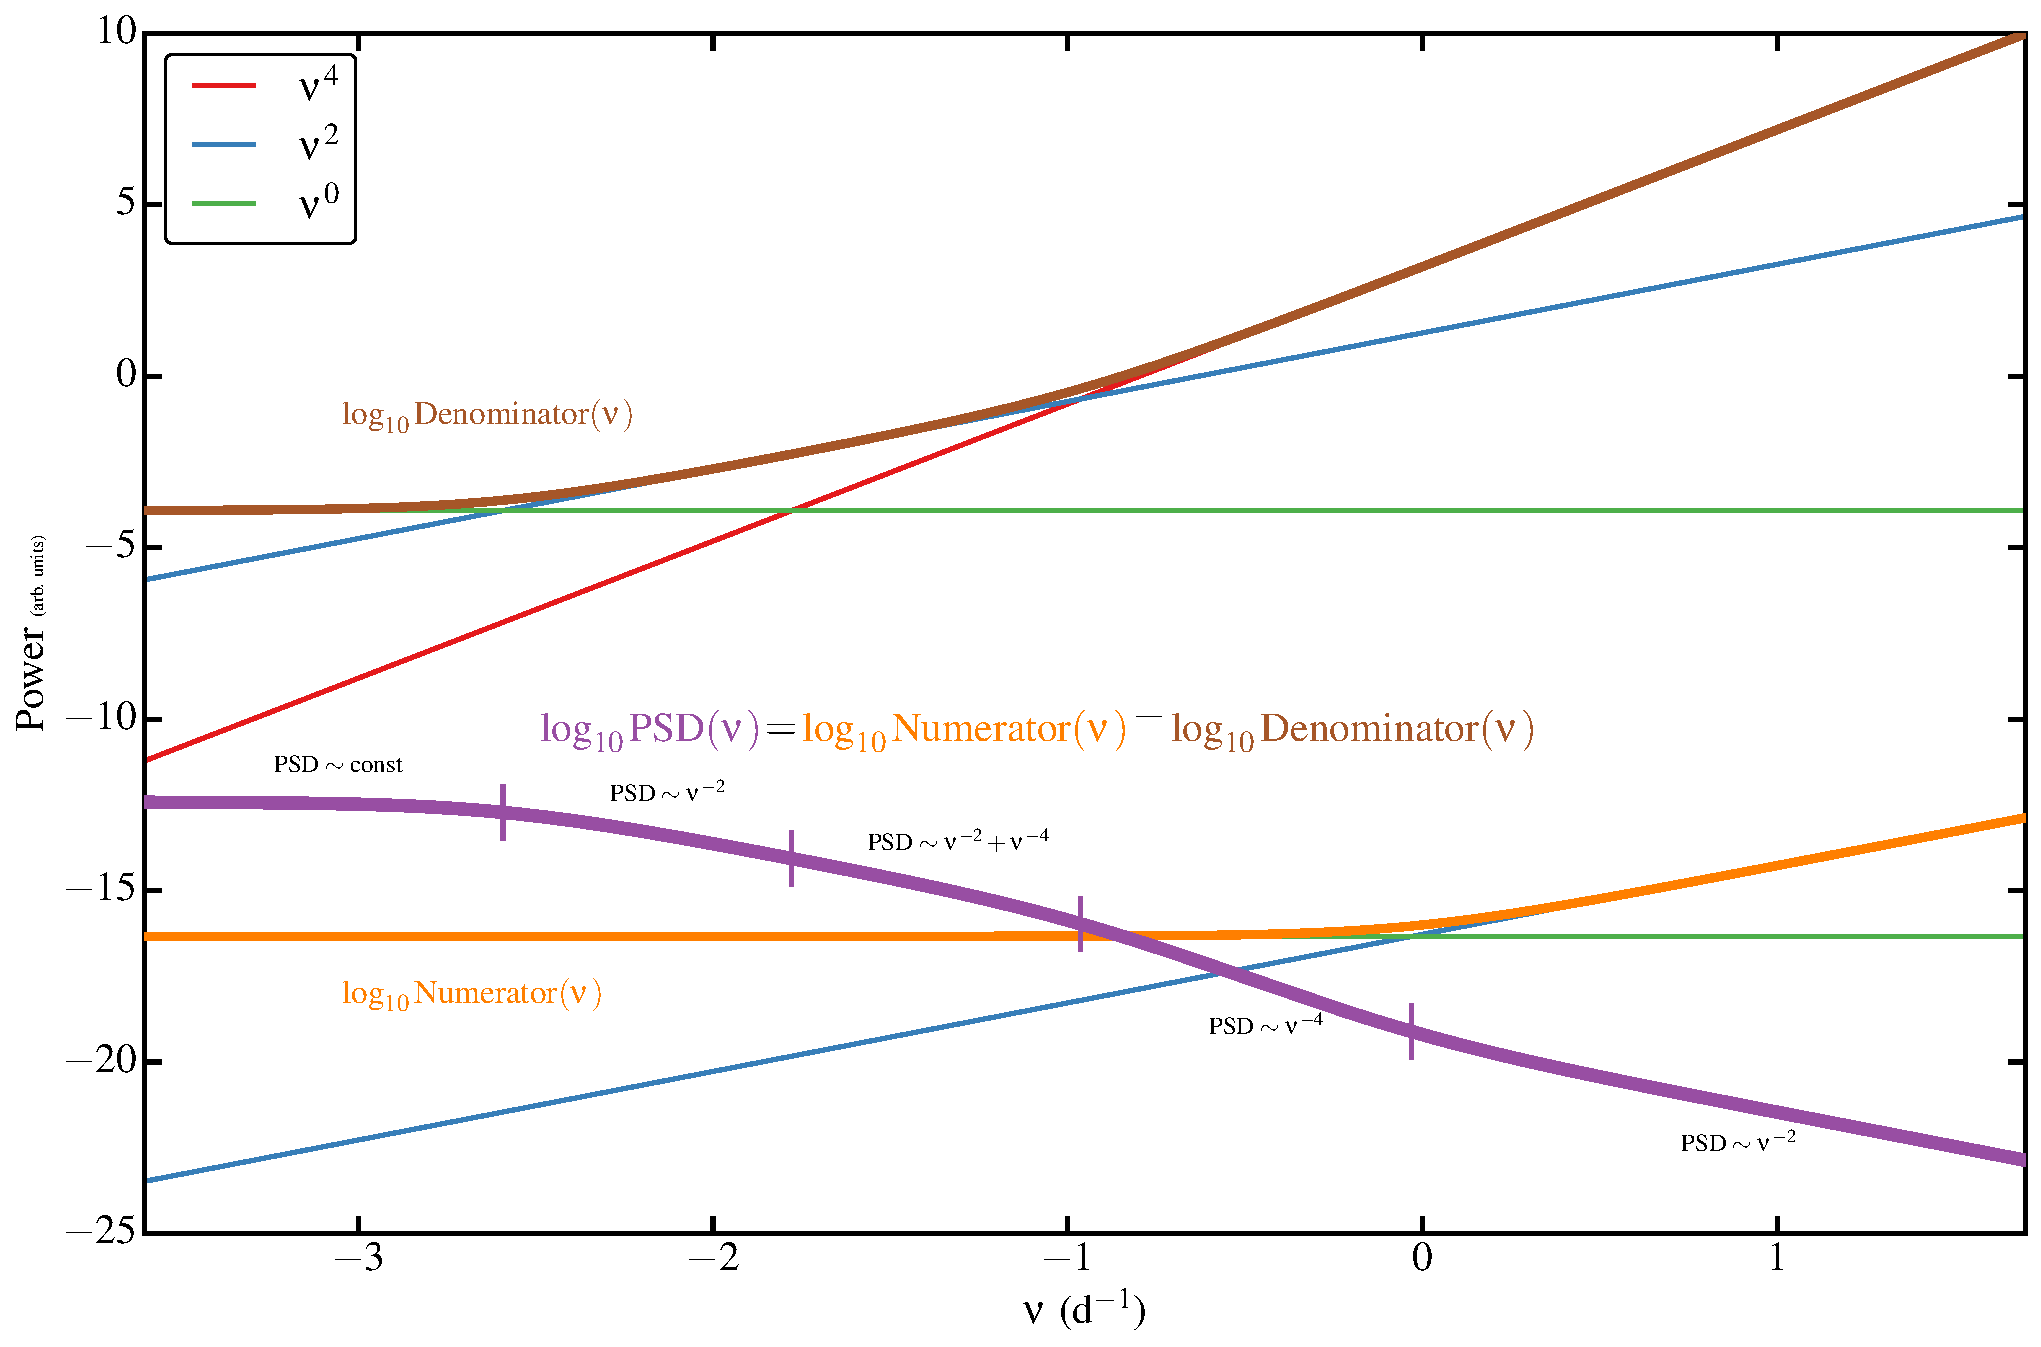
\includegraphics[width=5.0in]{figs/agn/AGN_Variability_01.pdf}
\caption{Behavior of the spectral index of the PSD (black) of the Kepler Sy1 
AGN Zw 229-15. This AGN is well-modelled by a C-ARMA(2,1) process. The spectral index varies
from 0 to 4 depending upon the frequency. Insufficient sampling of the light
curve (e.g. a few times a month), can result in the erroneous conclusion that a 
damped random walk (DRW) model (max spectral slope 2), adequately 
characterizes the variability.
}
\label{PSDvsFreq}
\end{figure}

Determination of the hyperparmeters that describe the PSD requires high frequency
sampling of the light curve ($\sim 1$~d$^{-1}$). Figure \ref{PSDvsFreq} shows
the frequency dependence of the spectral index of the PSD (black) of the Kepler Sy 1 AGN 
Zw 229-15. The light curve of this AGN is well-modelled by a C-ARMA(2,1) 
model. The C-ARMA(2,1) is a higher order random walk than the 
Damped Random Walk (DRW) of \citet{Kelly09} which is a C-ARMA(1,0)
 model. Recent varaibility studies indicate that the simple C-ARMA(1,0) 
model is insufficient to model AGN variability because the spectral
 index of the C-ARMA(1,0)
model is mathematically constrained to be 2 \citep{Kelly14,Kasliwal15,Simm15}. 
The PSD (black line) is the ratio of an even polynomial numerator (orange line) to 
an even polynomial denominator (brown line). Different powers of frequency dominate
the PSD at different frequencies depending on the hyperparameters of the C-ARMA(2,1) model. It is
clear that in the case of this AGN, the light curve must be sampled on timescales {\em shorter} than 
$1$-$5$ days in order to observe the $\nu^{-4}$ behavior characteristic of a higher order random walk.

\begin{figure}
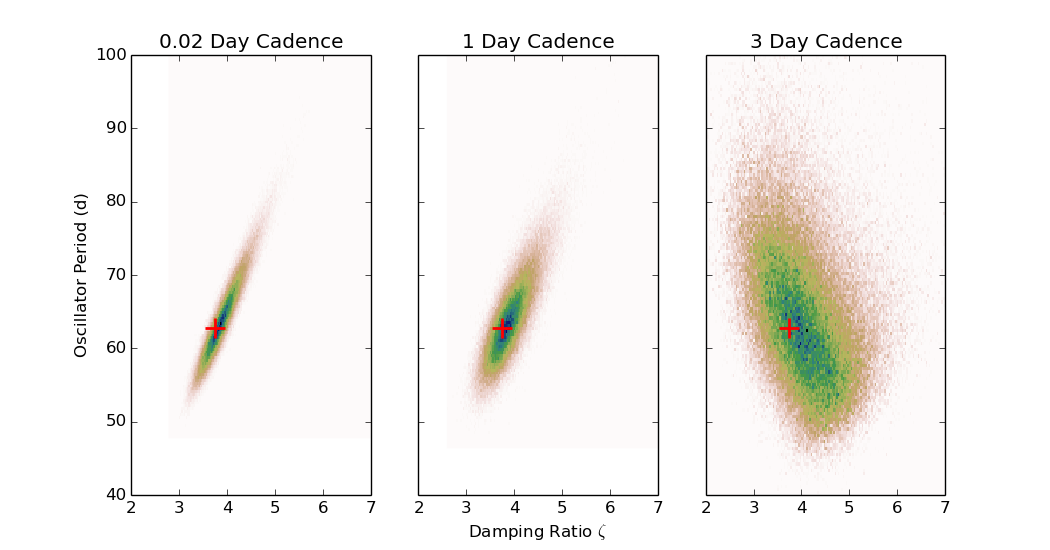
\includegraphics[width=5.0in]{figs/agn/AGN_Variability_00.png}
\caption{The effect of sampling cadence on hyperparameter estimation.}
\label{CadenceEffec}
\end{figure}

Accurate recovery of the PSD hyperparameters is greatly enhanced by rapid sampling. Figure \ref{CadenceEffect}
shows the effect of the sampling frequency on the inferred joint distribution of two
 hyperparameters of the C-ARMA(2,1) model, the 
oscillator timescale and the damping ratio. Degrading the sampling frequency from $1/$($30$~min) 
(Kepler) to $1/$($3$~d) changes both the size and the shape of the joint distribution i.e. it degrades both 
the accuracy and correlation of the inferred hyperparameters. 

The PRM measurements will probe the size and structure of the
accretion disk and BELR, in a statistical sense, and may provide
improved SMBH mass estimates for sources that have at least
single-epoch spectra. \new{Our goal is to understand the population of
AGN broad line regions, including their geometry. We expect to do this
via  a model that connects the BH mass, BLR geometry and AGN
photometric variability properties via a set of scaling relations. A
simple version of this is could be something like...\newline\newline
So, our target measurements are of $a$ and $b$, the X parameters.
Before we derive a metric that quantifies our ability to measure these
parameters, we can anticipate some of the sensitivity of the
photometric RM method to observing strategy.}

The PRM method is very sensitive to the sampling in each band,
therefore the ability to derive reliable time delays can be affected
significantly by the LSST cadence. The best results will be obtained
by having the most uniform sampling equally for each band.
Additionally, there is a trade-off between the number of DDFs and the
number of time delays that PRM can obtain \citep{CheloucheEtal2014}.
For example, an increase in the number of DDFs, with similarly dense
sampling in each field, can yield a proportionately larger number of
high-quality time delays, down to lower luminosities, but at the
expense of far fewer time delays (for relatively high luminosity
sources) in the main survey.

%\new{We focus on the PSD function as a way of characterizing AGN
%variability in various ways. What do we expect the AGN population to
%look like in PSD parameter space? The hyper-parameters that govern the
%relationships between PSD parameters and  AGN and host galaxy
%properties are probably of greatest scintific interest.}

% --------------------------------------------------------------------

\subsection{Metrics}
\label{sec:\secname:metrics}

Quantifying the response via MAF metrics: definition of the metrics,
and any derived overall figure of merit.

\new{In lieu of a simulated AGN population, we focus on a few
particular {\it diagnostic} metrics that capture  our likely ability
to measure the PSD across the population. These include: the
uniformity of the sampling pattern in log time lag?}


Need to compute the average and the dispersion in the
number of visits, per band, across the sky for the nominal OpSim
(during the entire survey). Since PRM works best for uniform sampling,
need to compare the distributions of the number of visits in each
band, averaged across the sky, and identify ways to minimize any
potential differences between these distributions. By running PRM
simulations, identify the 1) minimum number of visits (in any band)
that can yield any meaningful BELR-continuum lag estimates, and 2) the
largest difference in the number of visits between two different bands
that can yield any meaningful BELR-continuum lag estimates. Repeat
these simulations by doubling the nominal number of DDFs. Assess the
number of meaningful BELR-continuum time delays that can be obtained
with the nominal OpSim, and point out potential perturbations in the
cadence to improve the number and quality of such time delays.

% QPOs - Will the cadence and duration give you the proper range on the
% power spectrum to detect QPOs with a given mass, spin, and L/Ledd?
% (Bob Wagoner)


% --------------------------------------------------------------------

\subsection{OpSim Analysis}
\label{sec:\secname:analysis}

OpSim analysis: how good would the default observing strategy be, at
the time of writing for this science project?


% --------------------------------------------------------------------

\subsection{Discussion}
\label{sec:\secname:discussion}

Discussion: what risks have been identified? What suggestions could be
made to improve this science project's figure of merit, and mitigate
the identified risks?


% ====================================================================

\navigationbar
